\documentclass[12pt]{article}
\usepackage[slovene]{babel}
\usepackage[utf8]{inputenc}
\usepackage[T2A]{fontenc}
\usepackage{amsmath}
\usepackage{amsfonts}
\usepackage{amssymb}
\usepackage[version=4]{mhchem}
\usepackage{stmaryrd}
\usepackage{graphicx}
\usepackage[export]{adjustbox}
\graphicspath{ {./images/} }
\usepackage{physics}
\usepackage{geometry}
\geometry{left=2cm,right=2cm,top=2cm,bottom=2cm}
\usepackage{pgfplots}
\pgfplotsset{compat=1.18}
\usepackage{tikz}
\usetikzlibrary{arrows.meta}
\usetikzlibrary{backgrounds}
\usepgfplotslibrary{patchplots}
\usepgfplotslibrary{fillbetween}
\pgfplotsset{%
    layers/standard/.define layer set={%
        background,axis background,axis grid,axis ticks,axis lines,axis tick labels,pre main,main,axis descriptions,axis foreground%
    }{
        grid style={/pgfplots/on layer=axis grid},%
        tick style={/pgfplots/on layer=axis ticks},%
        axis line style={/pgfplots/on layer=axis lines},%
        label style={/pgfplots/on layer=axis descriptions},%
        legend style={/pgfplots/on layer=axis descriptions},%
        title style={/pgfplots/on layer=axis descriptions},%
        colorbar style={/pgfplots/on layer=axis descriptions},%
        ticklabel style={/pgfplots/on layer=axis tick labels},%
        axis background@ style={/pgfplots/on layer=axis background},%
        3d box foreground style={/pgfplots/on layer=axis foreground},%
    },
}

\title{\textbf{Sklopljena nihajna kroga}}
\author{Samo Krejan}
\date{maj 2025}

\begin{document}
\maketitle

\section{Uvod}

Zelo pogosto se v naravi srečamo s pojavi, kjer gre za dva ali več nihal, ki so med seboj sklopljena. Zaradi omenjene sklopitvije nihal ne moremo več obravnavati ločeno temveč kot en sistem.

Sistem $n$ enakih in enostavnih oscilatorjev ima $n$ lastnih nihanj. V prvem letniku smo že spoznali obnašanje dveh sklopljenih fizičnih nihal; tam sta lastni frekvenci ko nihali nihata točno v fazi in ko nihata iz faze. Prva lastna frekvenca je kar enaka lastni frekvenci posameznega nihala, druga pa je hitrejša, če je sklopitev močnejša.

Pri tej vaji smo opazovali električna nihajna kroga sklopljena s kondenzatorjem. En sam nihajni krog sestavljen iz kondenzatorja s kapaciteto $C$ in tuljave z induktivnostjo $L$ niha s krožno frekvenco; 

$$\omega_0 = \frac{1}{\sqrt{LC}}$$

Če je v nihajnem krogu prisoten še upor $R$, nastopi dušenje, ki ga opišemo s koeficientom $\beta = R/2L$. Sistem opisujejo enačbe za dušeno nihanje z rešitvijo;

$$I(t) = e^{-\beta t} \left(I_1\sin{\omega ' t} + I_2\cos{\omega ' t}\right)$$

Kjer je $\omega ' = \sqrt{\omega_0^2 - \beta^2}$

Če k prvemu krogu vežemo še drugi preko kondenzatorja $C_0$ potem dobimo sklopljen sistem nihajnih krogov. zaradi dveh prostorskih stopenj imamo torej dva lastna načina nihanja; prvi je enak kot prej, ko oba nihata v fazi, drugi lasten način pa je:

$$U_{1,2} = \pm U_0 e^{-\beta t} \cos (\omega '' t)$$

kjer je $\omega '' = \sqrt{\frac{C}{C-C_0}\omega_0^2 - \beta^2}$.

Splošno obnašanje sistema lahko opišemo kot linearno kombinacijo obeh lastnih nihanj:

$$U_{1,2} = e^{-\beta t} \left(U' \cos (\omega' t) \pm U'' \cos (\omega '' t + \delta)\right)$$



\section{Potrebščine}

\begin{itemize}
\item Digitalni osciloskop,
\item funkcijski generator napetosti, namizni multimeter,
\item nihajna kroga in kabli, USB ključek,
\item prenosnik z ustrezno programsko opremo.
\end{itemize}


\section{Naloga}

\begin{enumerate}
\item Izmerite časovni potek napetosti na obeh krogih pri vzbujanju s stopničastim signalom za vse različne sklopitve,
\item Izmerite frekvenčno karakteristiko enega nihajnega kroga in določite dobroto $Q$
\item Izmerite frekvenčo karakteristiko sklopljenih nihajnih krogov z meritvijo odziva drugega kroga za vsak $C_0$ in izmerite razliko lastnih krožnih frekvenc
\end{enumerate}


\section{Rezultati in analiza}

Nihajna kroga sta sestavljena iz tuljave z induktivnostjo $L$, kondenzatorja s kapacitivnostjo $C = 5.6\ nF$ in uporom z upornostjo $R = 7.5\ \Omega$. Najprej smo priklopili nihajna kroga na osciloskop in vir stopničaste napetosti (glej sliko vezja). Izmerili smo odziv prvega in drugega kondenzatorja pri vseh različnih sklopitvah.

\begin{figure}[ht]
\begin{center}
    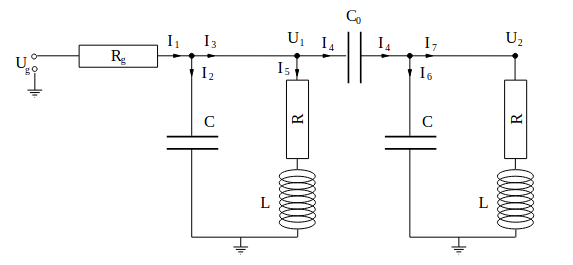
\includegraphics[width=10cm]{vezje.png}
    \caption{Skica vezja uporabljenega pri eksperimentu}
\end{center}
\end{figure}

Najprej smo merili odziv brez sklopitve $C_0 = 0$, a se je že tu izkazalo, da je prišlo do nekaj sklopitve. Tako smo že tu na grafa $U_1, U_2$ že na tej točki *fitali* funkciji:

$$U_1(t) = U_0 e^{-\beta t} \sin \left(\frac{\omega ' + \omega''}{2}t\right)\cos\left((\omega'-\omega'')t\right)$$

$$U_2(t) = U_0 e^{-\beta t} \sin \left(\frac{\omega ' + \omega''}{2}t\right)\sin\left((\omega'-\omega'')t\right)$$

Če bi na grafe risali tudi fite funkcij bi nastal kaos, tako da smo poleg izmerjenih podatkov risali zgolj ovojnico. Na ta način smo dobili naslednja grafa:
\newpage

\begin{figure}[h]
\centering
\begin{minipage}[t]{0.45\textwidth}
    \includegraphics[width=\textwidth]{p1.pdf}

\end{minipage}
\hfill
\begin{minipage}[t]{0.45\textwidth}
    \includegraphics[width=\textwidth]{p2.pdf}

\end{minipage}
\caption{$U_1, U_2$ izmerjena, ter njuni ovojnici pri minimalni sklopitvi}
\end{figure}

Iz fita dobimo vrednosti parametra $\omega' = 4.2\cdot 10^5 \ 1/s$, napake fita pa tu ne bom navajal, saj je manjša od procenta. Če predpostavimo $\omega >> \beta$ (kar lahko naredimo saj mo daleč od kritičnega dušenja), dobimo $L = 9.9\cdot 10^{-4} H$ Za tem smo praktično isti postopek ponovili še za ostale sklopitve. Primer meritve in ovojnice fita vidimo na naslednjih dveh grafih:

\begin{figure}[h]
\centering
\begin{minipage}[t]{0.45\textwidth}
    \includegraphics[width=\textwidth]{p3.pdf}

\end{minipage}
\hfill
\begin{minipage}[t]{0.45\textwidth}
    \includegraphics[width=\textwidth]{p4.pdf}

\end{minipage}
\caption{$U_1, U_2$ izmerjena, ter njuni ovojnici pri minimalni sklopitvi}
\end{figure}
Ko smo tako fitali omenjeno funkcijo na podatke smo dobili naslednje vrednosti predstavljene v tabeli:

\begin{table}[!ht]
\centering
\begin{tabular}{c|c|c|c}
    $C$ [$pF$] & krog & $\beta$ [$s^{-1}$] & $\Delta  \omega$ [$s^{-1}$] \\\hline \hline

    $330$ & $U_1$ & $6262 \pm 2$ & $18996 \pm 2$\\
    & $U_2$ & $6585\pm 2$ & $18887 \pm 1$\\
    $560$ & $U_1$ & $6080\pm 2$ & $26368\pm 2$\\
    & $U_2$ & $6347\pm 2$ & $26302\pm 1$\\
    $820$ & $U_1$ & $5976\pm 2$ & $33644\pm 2$\\
    & $U_2$ & $6200\pm 2$ & $33600\pm 1$\\
    $1150$ &$U_1$ & $6252\pm 1$ & $40368\pm 1$\\
    & $U_2$ & $6430\pm 2$ & $40338\pm 1$\\\hline \hline
    povprečje && $6300\pm 300$ &
\end{tabular}
\caption{Tabela izmerjenih vrednosti}
\end{table}
kjer je $\Delta \omega = \omega' - \omega''$. Če $\beta$ izračunamo iz podanega upora in prej izračunane induktivnosti dobimo:

$$
\beta' = \frac{R}{2L} = 3787\ s^{-1}
$$
kar zelo močno odstopa od izmerjene vrednosti. Razlog za to je v morda večjem uporu, ali kakšni drugi neidealizaciji. Frekvence utripanja smo nato nanesli na graf v odvsnosti od sklopitvenega kondenzatorja:

% Recommended preamble:
% \usetikzlibrary{arrows.meta}
% \usetikzlibrary{backgrounds}
% \usepgfplotslibrary{patchplots}
% \usepgfplotslibrary{fillbetween}
% \pgfplotsset{%
%     layers/standard/.define layer set={%
%         background,axis background,axis grid,axis ticks,axis lines,axis tick labels,pre main,main,axis descriptions,axis foreground%
%     }{
%         grid style={/pgfplots/on layer=axis grid},%
%         tick style={/pgfplots/on layer=axis ticks},%
%         axis line style={/pgfplots/on layer=axis lines},%
%         label style={/pgfplots/on layer=axis descriptions},%
%         legend style={/pgfplots/on layer=axis descriptions},%
%         title style={/pgfplots/on layer=axis descriptions},%
%         colorbar style={/pgfplots/on layer=axis descriptions},%
%         ticklabel style={/pgfplots/on layer=axis tick labels},%
%         axis background@ style={/pgfplots/on layer=axis background},%
%         3d box foreground style={/pgfplots/on layer=axis foreground},%
%     },
% }

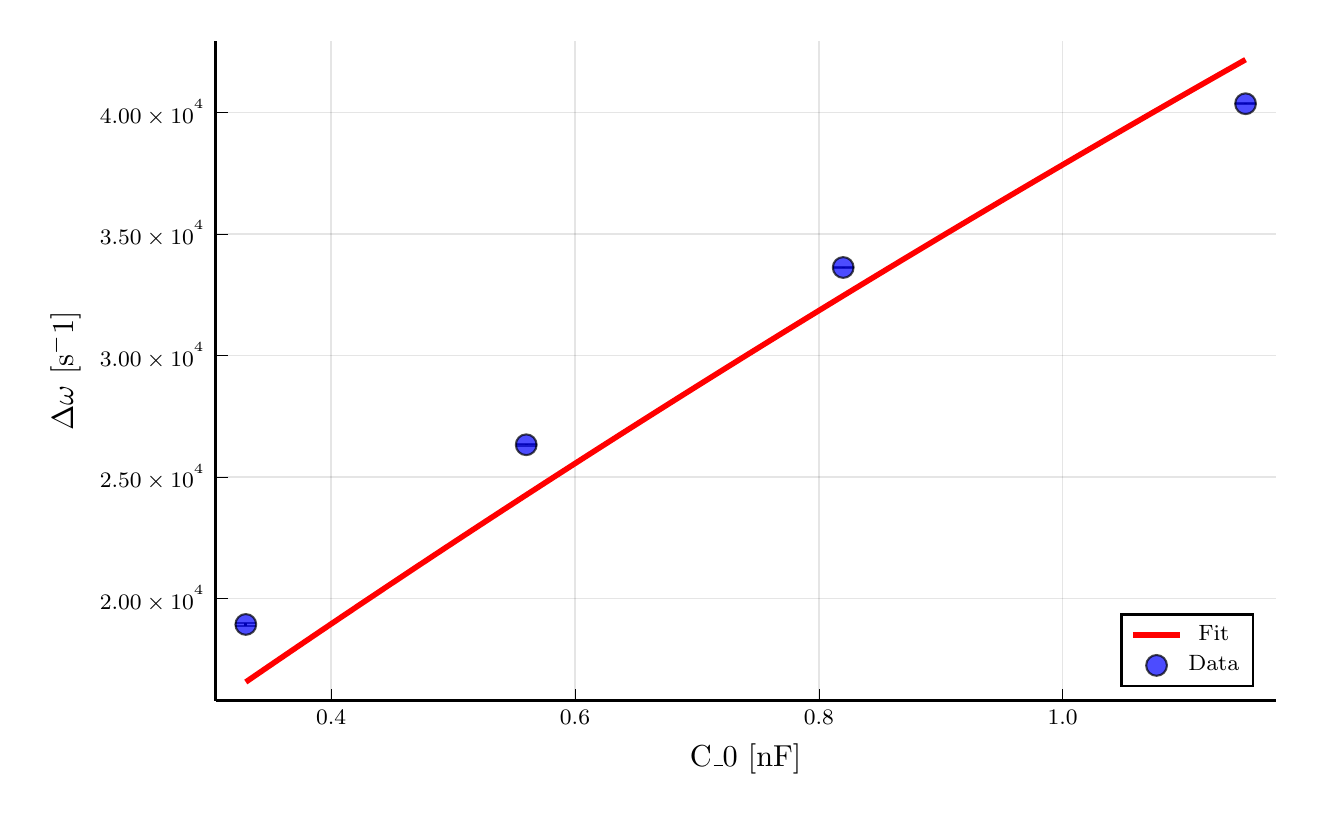
\begin{tikzpicture}[/tikz/background rectangle/.style={fill={rgb,1:red,1.0;green,1.0;blue,1.0}, fill opacity={1.0}, draw opacity={1.0}}, show background rectangle]
\begin{axis}[point meta max={nan}, point meta min={nan}, legend cell align={left}, legend columns={1}, title={}, title style={at={{(0.5,1)}}, anchor={south}, font={{\fontsize{14 pt}{18.2 pt}\selectfont}}, color={rgb,1:red,0.0;green,0.0;blue,0.0}, draw opacity={1.0}, rotate={0.0}, align={center}}, legend style={color={rgb,1:red,0.0;green,0.0;blue,0.0}, draw opacity={1.0}, line width={1}, solid, fill={rgb,1:red,1.0;green,1.0;blue,1.0}, fill opacity={1.0}, text opacity={1.0}, font={{\fontsize{8 pt}{10.4 pt}\selectfont}}, text={rgb,1:red,0.0;green,0.0;blue,0.0}, cells={anchor={center}}, at={(0.98, 0.02)}, anchor={south east}}, axis background/.style={fill={rgb,1:red,1.0;green,1.0;blue,1.0}, opacity={1.0}}, anchor={north west}, xshift={1.0mm}, yshift={-1.0mm}, width={150.4mm}, height={99.6mm}, scaled x ticks={false}, xlabel={C\_0 [nF]}, x tick style={color={rgb,1:red,0.0;green,0.0;blue,0.0}, opacity={1.0}}, x tick label style={color={rgb,1:red,0.0;green,0.0;blue,0.0}, opacity={1.0}, rotate={0}}, xlabel style={at={(ticklabel cs:0.5)}, anchor=near ticklabel, at={{(ticklabel cs:0.5)}}, anchor={near ticklabel}, font={{\fontsize{11 pt}{14.3 pt}\selectfont}}, color={rgb,1:red,0.0;green,0.0;blue,0.0}, draw opacity={1.0}, rotate={0.0}}, xmajorgrids={true}, xmin={0.30540000000000006}, xmax={1.1746}, xticklabels={{$0.4$,$0.6$,$0.8$,$1.0$}}, xtick={{0.4,0.6000000000000001,0.8,1.0}}, xtick align={inside}, xticklabel style={font={{\fontsize{8 pt}{10.4 pt}\selectfont}}, color={rgb,1:red,0.0;green,0.0;blue,0.0}, draw opacity={1.0}, rotate={0.0}}, x grid style={color={rgb,1:red,0.0;green,0.0;blue,0.0}, draw opacity={0.1}, line width={0.5}, solid}, axis x line*={left}, x axis line style={color={rgb,1:red,0.0;green,0.0;blue,0.0}, draw opacity={1.0}, line width={1}, solid}, scaled y ticks={false}, ylabel={$\Delta$$\omega$ [s$^-$1]}, y tick style={color={rgb,1:red,0.0;green,0.0;blue,0.0}, opacity={1.0}}, y tick label style={color={rgb,1:red,0.0;green,0.0;blue,0.0}, opacity={1.0}, rotate={0}}, ylabel style={at={(ticklabel cs:0.5)}, anchor=near ticklabel, at={{(ticklabel cs:0.5)}}, anchor={near ticklabel}, font={{\fontsize{11 pt}{14.3 pt}\selectfont}}, color={rgb,1:red,0.0;green,0.0;blue,0.0}, draw opacity={1.0}, rotate={0.0}}, ymajorgrids={true}, ymin={15804.308058201192}, ymax={42935.82953491232}, yticklabels={{$2.00\times10^{^{4}}$,$2.50\times10^{^{4}}$,$3.00\times10^{^{4}}$,$3.50\times10^{^{4}}$,$4.00\times10^{^{4}}$}}, ytick={{20000.0,25000.0,30000.0,35000.0,40000.0}}, ytick align={inside}, yticklabel style={font={{\fontsize{8 pt}{10.4 pt}\selectfont}}, color={rgb,1:red,0.0;green,0.0;blue,0.0}, draw opacity={1.0}, rotate={0.0}}, y grid style={color={rgb,1:red,0.0;green,0.0;blue,0.0}, draw opacity={0.1}, line width={0.5}, solid}, axis y line*={left}, y axis line style={color={rgb,1:red,0.0;green,0.0;blue,0.0}, draw opacity={1.0}, line width={1}, solid}, colorbar={false}]
    \addplot[color={rgb,1:red,1.0;green,0.0;blue,0.0}, name path={1}, draw opacity={1.0}, line width={2}, solid]
        table[row sep={\\}]
        {
            \\
            0.33  16572.181307542076  \\
            0.3382828282828283  16856.949593394584  \\
            0.3465656565656566  17141.122718615803  \\
            0.35484848484848486  17424.70275349379  \\
            0.36313131313131314  17707.691758248835  \\
            0.3714141414141414  17990.09178309544  \\
            0.3796969696969697  18271.904868305366  \\
            0.387979797979798  18553.13304426928  \\
            0.39626262626262626  18833.77833155816  \\
            0.4045454545454546  19113.84274098434  \\
            0.4128282828282829  19393.328273662246  \\
            0.42111111111111116  19672.23692106787  \\
            0.42939393939393944  19950.570665098898  \\
            0.4376767676767677  20228.331478133794  \\
            0.445959595959596  20505.521323090183  \\
            0.4542424242424243  20782.142153483637  \\
            0.46252525252525256  21058.1959134849  \\
            0.47080808080808084  21333.684537977675  \\
            0.4790909090909091  21608.60995261557  \\
            0.4873737373737374  21882.974073878428  \\
            0.4956565656565657  22156.778809128733  \\
            0.503939393939394  22430.02605666697  \\
            0.5122222222222222  22702.717705787156  \\
            0.5205050505050506  22974.855636831544  \\
            0.5287878787878788  23246.441721245235  \\
            0.5370707070707071  23517.47782163013  \\
            0.5453535353535354  23787.9657917986  \\
            0.5536363636363637  24057.9074768268  \\
            0.5619191919191919  24327.30471310735  \\
            0.5702020202020203  24596.159328402075  \\
            0.5784848484848485  24864.473141893857  \\
            0.5867676767676768  25132.24796423857  \\
            0.595050505050505  25399.485597616116  \\
            0.6033333333333334  25666.187835781482  \\
            0.6116161616161617  25932.35646411555  \\
            0.61989898989899  26197.993259674924  \\
            0.6281818181818183  26463.09999124199  \\
            0.6364646464646465  26727.678419374333  \\
            0.6447474747474748  26991.73029645375  \\
            0.6530303030303031  27255.257366735135  \\
            0.6613131313131314  27518.261366394985  \\
            0.6695959595959596  27780.744023578936  \\
            0.677878787878788  28042.707058450145  \\
            0.6861616161616162  28304.152183236085  \\
            0.6944444444444445  28565.081102275868  \\
            0.7027272727272728  28825.49551206664  \\
            0.7110101010101011  29085.39710131037  \\
            0.7192929292929293  29344.78755095921  \\
            0.7275757575757577  29603.668534261753  \\
            0.7358585858585859  29862.041716807984  \\
            0.7441414141414142  30119.908756574438  \\
            0.7524242424242426  30377.27130396885  \\
            0.7607070707070708  30634.131001874626  \\
            0.7689898989898991  30890.489485694674  \\
            0.7772727272727273  31146.348383395347  \\
            0.7855555555555557  31401.70931554981  \\
            0.7938383838383839  31656.573895381003  \\
            0.8021212121212122  31910.943728804643  \\
            0.8104040404040405  32164.820414471727  \\
            0.8186868686868688  32418.205543810614  \\
            0.826969696969697  32671.100701068815  \\
            0.8352525252525254  32923.50746335496  \\
            0.8435353535353536  33175.427400679786  \\
            0.8518181818181819  33426.86207599728  \\
            0.8601010101010101  33677.81304524547  \\
            0.8683838383838385  33928.28185738663  \\
            0.8766666666666667  34178.27005444781  \\
            0.884949494949495  34427.7791715603  \\
            0.8932323232323234  34676.81073699949  \\
            0.9015151515151516  34925.366272224106  \\
            0.9097979797979799  35173.447291915414  \\
            0.9180808080808082  35421.05530401563  \\
            0.9263636363636365  35668.191809766686  \\
            0.9346464646464647  35914.85830374847  \\
            0.9429292929292931  36161.05627391667  \\
            0.9512121212121213  36406.787201640596  \\
            0.9594949494949496  36652.052561740384  \\
            0.9677777777777778  36896.853822524536  \\
            0.9760606060606062  37141.19244582648  \\
            0.9843434343434344  37385.069887041456  \\
            0.9926262626262627  37628.48759516293  \\
            1.000909090909091  37871.447012818644  \\
            1.0091919191919192  38113.94957630656  \\
            1.0174747474747476  38355.996715630514  \\
            1.0257575757575759  38597.58985453564  \\
            1.034040404040404  38838.73041054367  \\
            1.0423232323232325  39079.41979498776  \\
            1.0506060606060608  39319.65941304707  \\
            1.058888888888889  39559.45066378131  \\
            1.0671717171717172  39798.79494016518  \\
            1.0754545454545457  40037.693629121924  \\
            1.0837373737373739  40276.14811155758  \\
            1.0920202020202021  40514.15976239408  \\
            1.1003030303030303  40751.72995060274  \\
            1.1085858585858588  40988.8600392373  \\
            1.116868686868687  41225.55138546682  \\
            1.1251515151515152  41461.80534060828  \\
            1.1334343434343435  41697.62325015896  \\
            1.141717171717172  41933.00645382859  \\
            1.1500000000000001  42167.95628557144  \\
        }
        ;
    \addlegendentry {Fit}
    \addplot[color={rgb,1:red,0.0;green,0.0;blue,0.0}, name path={2}, draw opacity={1.0}, line width={1}, solid, mark={-}, mark size={3.75 pt}, mark repeat={1}, mark options={color={rgb,1:red,0.0;green,0.0;blue,0.0}, draw opacity={0.7}, fill={rgb,1:red,0.0;green,0.0;blue,0.0}, fill opacity={0.7}, line width={0.75}, rotate={0}, solid}, forget plot]
        table[row sep={\\}]
        {
            \\
            0.33  18890.0  \\
            0.33  18990.0  \\
        }
        ;
    \addplot[color={rgb,1:red,0.0;green,0.0;blue,0.0}, name path={2}, draw opacity={1.0}, line width={1}, solid, mark={-}, mark size={3.75 pt}, mark repeat={1}, mark options={color={rgb,1:red,0.0;green,0.0;blue,0.0}, draw opacity={0.7}, fill={rgb,1:red,0.0;green,0.0;blue,0.0}, fill opacity={0.7}, line width={0.75}, rotate={0}, solid}, forget plot]
        table[row sep={\\}]
        {
            \\
            0.56  26300.0  \\
            0.56  26360.0  \\
        }
        ;
    \addplot[color={rgb,1:red,0.0;green,0.0;blue,0.0}, name path={2}, draw opacity={1.0}, line width={1}, solid, mark={-}, mark size={3.75 pt}, mark repeat={1}, mark options={color={rgb,1:red,0.0;green,0.0;blue,0.0}, draw opacity={0.7}, fill={rgb,1:red,0.0;green,0.0;blue,0.0}, fill opacity={0.7}, line width={0.75}, rotate={0}, solid}, forget plot]
        table[row sep={\\}]
        {
            \\
            0.8200000000000001  33590.0  \\
            0.8200000000000001  33650.0  \\
        }
        ;
    \addplot[color={rgb,1:red,0.0;green,0.0;blue,0.0}, name path={2}, draw opacity={1.0}, line width={1}, solid, mark={-}, mark size={3.75 pt}, mark repeat={1}, mark options={color={rgb,1:red,0.0;green,0.0;blue,0.0}, draw opacity={0.7}, fill={rgb,1:red,0.0;green,0.0;blue,0.0}, fill opacity={0.7}, line width={0.75}, rotate={0}, solid}, forget plot]
        table[row sep={\\}]
        {
            \\
            1.1500000000000001  40335.0  \\
            1.1500000000000001  40375.0  \\
        }
        ;
    \addplot[color={rgb,1:red,0.0;green,0.0;blue,1.0}, name path={3}, only marks, draw opacity={1.0}, line width={0}, solid, mark={*}, mark size={3.75 pt}, mark repeat={1}, mark options={color={rgb,1:red,0.0;green,0.0;blue,0.0}, draw opacity={0.7}, fill={rgb,1:red,0.0;green,0.0;blue,1.0}, fill opacity={0.7}, line width={0.75}, rotate={0}, solid}]
        table[row sep={\\}]
        {
            \\
            0.33  18940.0  \\
            0.56  26330.0  \\
            0.8200000000000001  33620.0  \\
            1.1500000000000001  40355.0  \\
        }
        ;
    \addlegendentry {Data}
\end{axis}
\end{tikzpicture}



\end{document}